
\section*{Results and discussion} % Kan også kaldes Results and Discussion. Og så kan Discussion (sek. 4 kaldes conclusion)


\subsection*{Overall distribution}
The overall distribution of copy numbers, across all genes and individuals, is shown in figure \ref{fig:qc_dist_all}. The distribution is near symmetrical, centered around a mean of 1.

% Figure 1
\begin{figure}[h] 
  \centering
  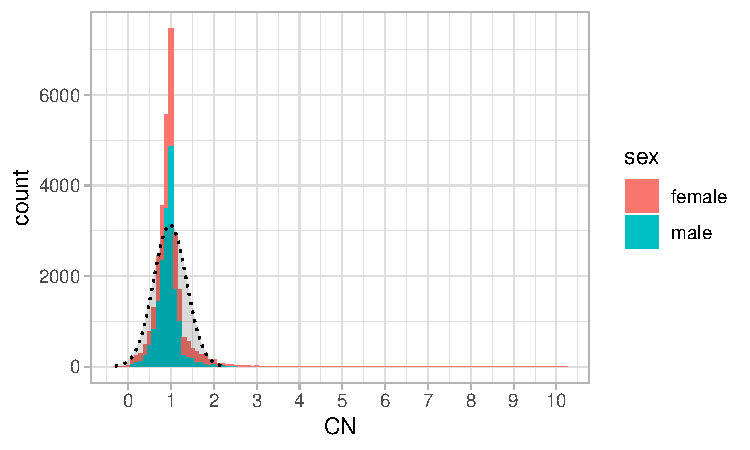
\includegraphics[width=0.58\textwidth]{figures/fig_qc_dist_all_1.pdf}
  
  \caption{Distribution of median CN across all genes for all subjects not including Simliki. A normal distribution with an equal mean, SD and area (grey) is overlapped as a visual aid. Colored by sex.}
  
  \label{fig:qc_dist_all}
\end{figure}

\noindent There is no known prior on the chromosome wide CN distribution. But a mean close to one makes good sense, as it suggests that linked paralogs have been described separately in the annotation. It also suggests, that the genes in the annotation have a representative length.

We checked that all individuals obey this distribution (figure \ref{fig:qc_subjects_simliki}), and observed that most individuals do. But, Simliki shows a chromosome wide CN median of 1.64, which suggests that Simliki's DMD gene has a size of $ \frac{100\%}{1.64} = 61\%} $ compared to the reference annotation. Failure to exclude Simliki from subsequent analysis might inflate the CN measurement. Thus, we decided to remove Simliki from subsequent analysis, and hypothesize, that Simliki's DMD gene might have a deletion. All other individuals have a chromosome wide median CN of less than 1.5, and are thus kept in the downstream analysis.??(fjernelse nævnt to gange) ??overvej også at teste forskel på køn med parret permutationstest.

Comparing the genes with the highest copy number variation with the results of Lucotte et al





% Figure 2
\begin{figure}[h] 
  \centering
  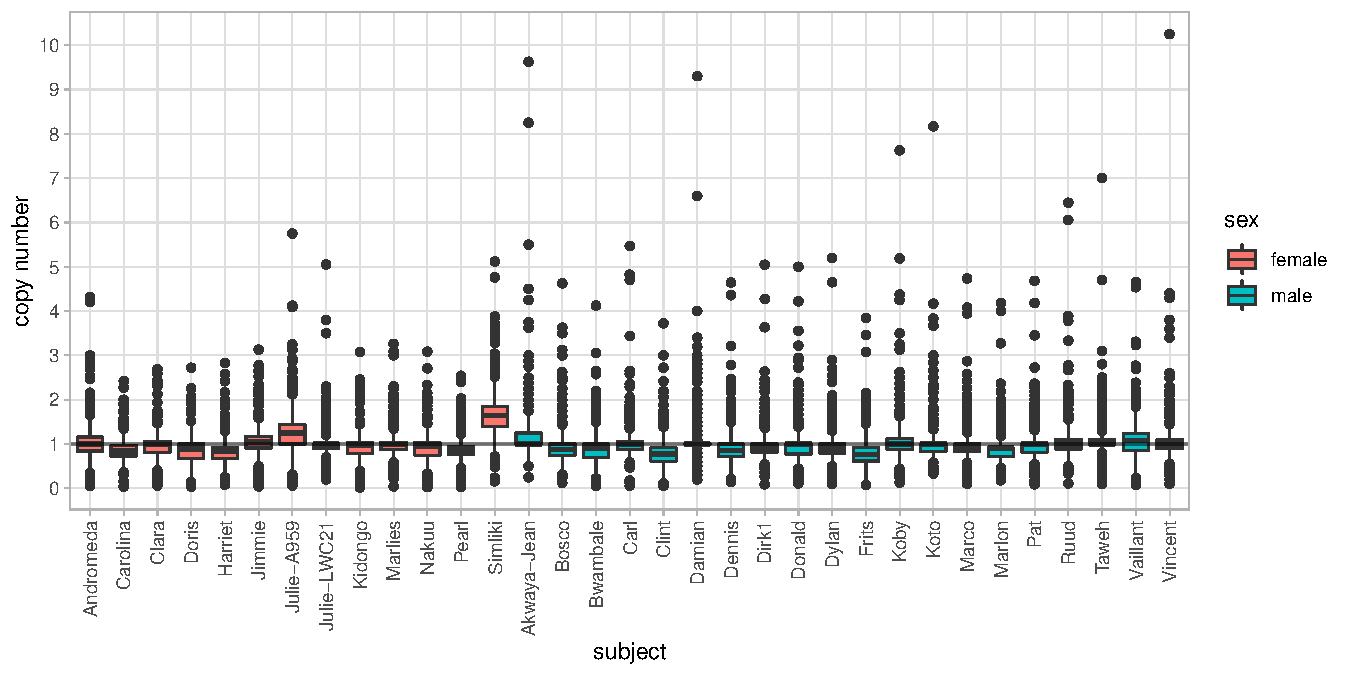
\includegraphics[scale=0.78]{figures/fig_qc_subjects_simliki_1.pdf}
  \caption{Distribution of median CN across all genes for each subject. Box edges denote quartiles. Points denote values beyond 1.5*IQR, where IQR is the interquartile range.}
  \label{fig:qc_subjects_simliki}
\end{figure}



%Some of the genes with the highest median copy numbers are overlapping. This spurred the hypothesis that 
\noindent Of the 919 genes on the X chromosome, 64 ({\raise.17ex\hbox{$\scriptstyle\sim$}}7\%) have an overlap with another gene. Performing a non-parametric (permutation) test on the difference (in means) of the distributions of medians for overlapping and non-overlapping genes, shows that the difference is not significantly different (\textit{p}-value = 0.1927).
Two genes, {\footnotesize CT55} and {\footnotesize TCP11x2} are duplicated in full length on the annotation, but since they each have relatively low variances (2nd quartile of overall SD), they are not considered actively ampliconic.

\subsection*{Checking paralogs on autosomes}
In this study, we map the reads to the X chromosome only. Because the rest of the chromosomes might contain paralogs of the genes on the X chromosome, it is relevant to check if the exclusion of the rest of the genome has a significant impact on the coverage of the genes on the X chromosome. In order to check this, we randomly picked a number of individuals (?? which) and compared the coverage of the X chromosome genes from this read mapping, to the read mapping of only the X chromosome. ??results




\subsection*{Most copy number-variant genes}


% Figure 3
\begin{figure}[h] 
  \centering
  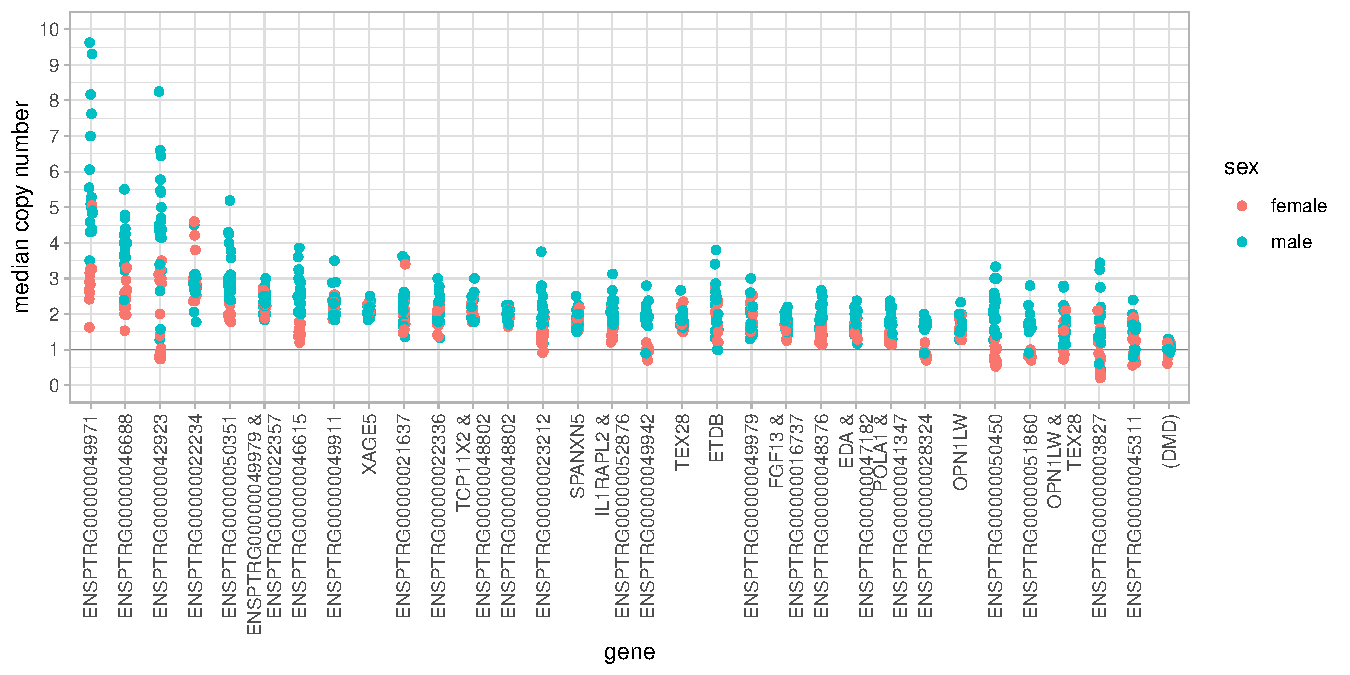
\includegraphics[scale=0.78]{figures/fig_main_median_3.pdf}
  \caption{Copy number from all subjects, grouped by genes. These 27 genes or overlaps of genes have a median copy number $\geq$ 1.5. Sorted by descending median. '\&' signifies the overlap of two genes. Horizontal jitter is applied. }
  \label{fig:fig_main}
\end{figure}


We looked up the genes with the highest median copy numbers. Unfortunately, many of the genes in the Pan\_tro\_3 reference genome are not named as exhaustively as in the human counterparts, and many of the genes thus have serial numbers instead. These serial numbers will be abbreviated as ENSPTRG00000049971 to E..49971. 
The genes with the highest median copy numbers are enumerated in figure \ref{fig:fig_main}.
\noindent E..49971, E..42923, E..46688,  E..22234, E..50351, E..49979, E..46615, E..49911, E..47182, E..48376, E..50450, E..49942, POLA1 have no obvious relation to anything meiosis related by name or description, and there is no expression data available. E..22357, XAGE5, E..22336,  is testis expressed but has no other description. E..21637 and OPN1LW have expression in several organs, where testis has the highest. EDA, FGF13 and E..41347 is expressed in several organs as well as the testis. TCP11X2, E..23212, TEX28 are testis expressed but has no other description. For E..48802, no Chimpanzee data is related, but an mRNA of an ortholog in Macaca Fascicularis is testis expressed. SPANXN5 has no expression data, but its description "Sperm protein associated with the nucleus on the X chromosome N1" suggests that it is expressed in the testis. ETDB has an identical homolog which is termed "Embryonic testis differentiation homolog", and thus suggests testis expression. E..52876 and E..16737 have no Chimpanzee expression data, but an ortholog in human with an identity of 90\% is testis expressed. E..28324 is not present in all subjects for unknown reasons. Nevertheless, has a median above 1.5, and is testis expressed.
\noindent Of the genes described in Lucotte et al. 2019, only {\footnotesize OPN1LW} is overlapping as a copy number-variant gene. Even though it codes for long-wavelength opsin in the retina, it has its highest expression in the testis according to the Bgee database (in Chimpanzee). Of the other genes in deemed copy number-variant Lucotte et al. 2019 - CT47A, presumably orthologous to ENSPTRG00000046894 "cancer/testis antigen 47A" has a max CN of 1.8 and a median CN of 0.9, and is thus not as variant in chimpanzee as in human (max CN: 15.07, median CN: 5.01). The other genes deemed copy number-variant in Lucotte et al. 2019 do not have identically named genes in the Chimpanzee annotation.
That is, assuming that the naming of the genes across the species is completely parsimonous. An alignment is necessary to be able to conclude that these are in fact orthologs.
\\



\noindent It seems like there is a relation between the high median CN and testis presence. As we don't know what proportion of the X-linked genes are expressed in the testis, it is hard to say if the genes with the highest variation are significantly more present in the testis. Nevertheless, for the genes where expression data was available, all genes but IL1RAPL2 showed signs of presence in the testis.






\\
\\
\noindent ??flyt højere op: Assuming that the genome wide CN median should be 1, suggests that it should be possible to convert the relative copy number measures to absolute by normalizing the subject-wise median to 1. Nonetheless, the DMD gene is a promising normalization candidate, as most subject get a median close to 1.

\\
\\
\subsection*{Copy number variation among relatives}
In order to investigate the copy number turnover between parents-offspring, we plotted the copy number over time measured in n'th degree relatives. For 7 of the 33?? Chimpanzees included in this study, we know the parent relation, and for 3 we know the grandparent relation. This means that we can compare the progression of copy numbers, down through the pedigree. In figure \ref{fig:pedigree_CN}, the copy numbers for the 5 most highly copied genes as well as OPN1LW is visualized. Dad-son relations are removed because no X chromosome is passed in this relation.

% Figure 4
\begin{figure}[h] 
  \centering
  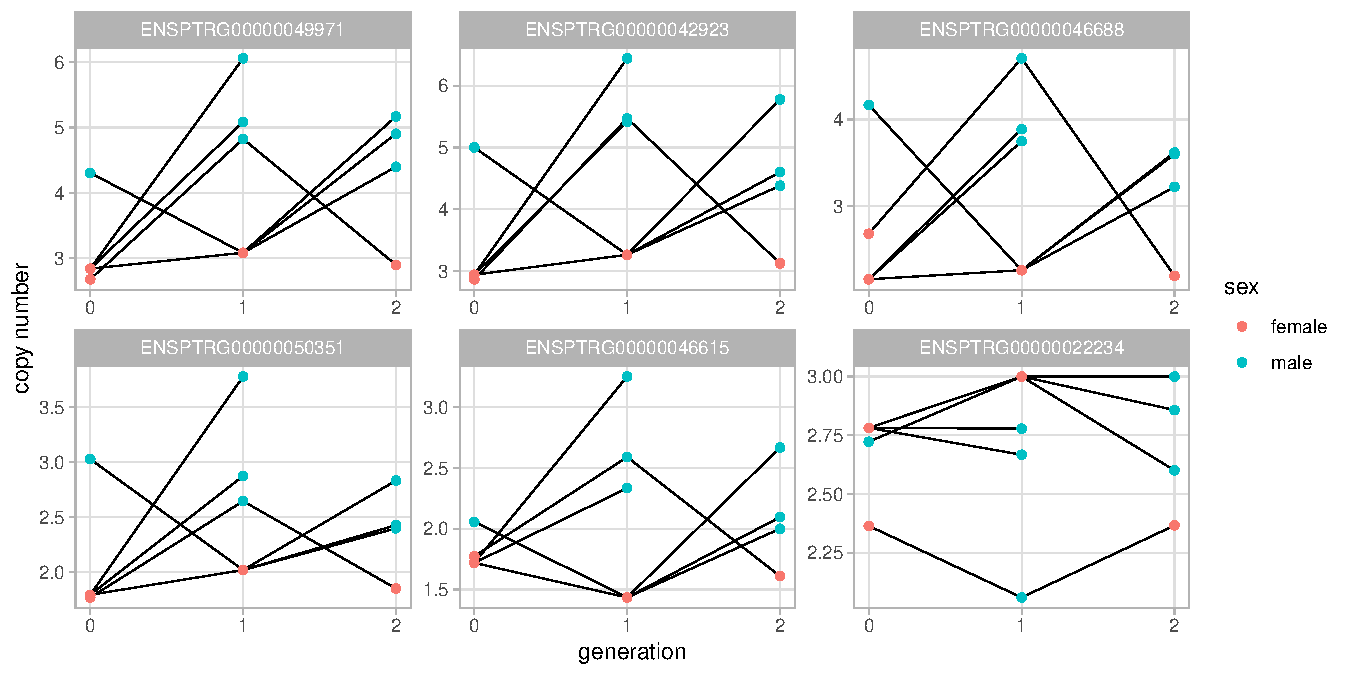
\includegraphics[scale=0.78]{figures/fig_pedigree_CN_3.pdf}
  \caption{Copy number as a function of pedigree. Each straight line denotes the change in copy number for an X-linked gene, when the X chromosome is passed from parent to offspring. Dad-son relations are not included.}
  \label{fig:pedigree_CN}
\end{figure}



